\documentclass[a4paper]{article}

\usepackage[spanish]{babel}
\usepackage{graphicx}
\usepackage{amsmath, amssymb}
\usepackage[margin=2cm]{geometry}
\usepackage{fancyhdr}
\usepackage{enumerate}
\usepackage[shortlabels]{enumitem}
\usepackage{parskip}
\usepackage[most]{tcolorbox}
\usepackage[hidelinks]{hyperref}
\usepackage{float}
\usepackage{setspace}
\usepackage{xspace}


\usepackage{tabularx}
\usepackage{ragged2e}
\newcolumntype{L}{>{\RaggedRight\arraybackslash}X}
\newcolumntype{C}{>{\Centering\arraybackslash}X}

% cabecera
\pagestyle{fancy}
\fancyhead[l]{Daniel Soto}
\fancyhead[c]{Problemas de Astronomía \#15}
\fancyhead[r]{\today}
\fancyfoot[c]{\thepage}
\renewcommand{\headrulewidth}{0.2pt} % linea horizontal

%% Definicion de comandos para formato de unidades fisicas %%
\newcommand{\m}{\text{m}}
\newcommand{\cm}{\text{cm}}
\newcommand{\mm}{\text{mm}}
\newcommand{\km}{\text{km}}
\newcommand{\s}{\text{s}}
\newcommand{\N}{\text{N}}
\newcommand{\g}{\text{g}}
\newcommand{\kg}{\text{kg}}
\newcommand{\Msolar}{\text{M}_\odot}
\newcommand{\Mterrestre}{\text{M}_\oplus}
\newcommand{\AU}{\text{AU}}
\newcommand{\ly}{\text{ly}}
\newcommand{\nT}{\text{nT}}
\newcommand{\keV}{\text{keV}}
\newcommand{\MeV}{\text{MeV}}
\newcommand{\GeV}{\text{GeV}}
\newcommand{\atoms}{\text{atoms}}
\newcommand{\K}{\text{K}}
\newcommand{\J}{\text{J}}
\newcommand{\particles}{\text{particles}}
\newcommand{\protones}{\text{p}^+}
\newcommand{\electrones}{\text{e}^-}
\newcommand{\Gy}{\text{Gy}}
\newcommand{\My}{\text{My}}
\newcommand{\nm}{\text{nm}}
\newcommand{\blank}{\rule{2cm}{0.4pt}\xspace}
\newcommand{\mol}{\text{mol}}
\newcommand{\W}{\text{W}}



\newcounter{problema}

\newtcolorbox[use counter=problema]{problema}[1][]{%
	breakable,
    colback=gray!15,
    colframe=gray!60,
    fonttitle=\bfseries,
    title={Problema~\theproblema:},
    boxrule=0.5mm,
    arc=3mm,
    boxsep=5pt,
    left=8pt,
    right=8pt,
    top=6pt,
    bottom=6pt,
    #1
}


\begin{document}

\begin{problema}

Modelos matemáticos detallados del interior del sol se basan en observaciones astronómicas y en nuestro conocimiento de la física de las estrellas. Estos modelos nos permiten explorar muchos aspectos de cómo 'funciona' el sol que están permanentemente ocultos a la vista.    

    \begin{figure}[H]
        \centering
        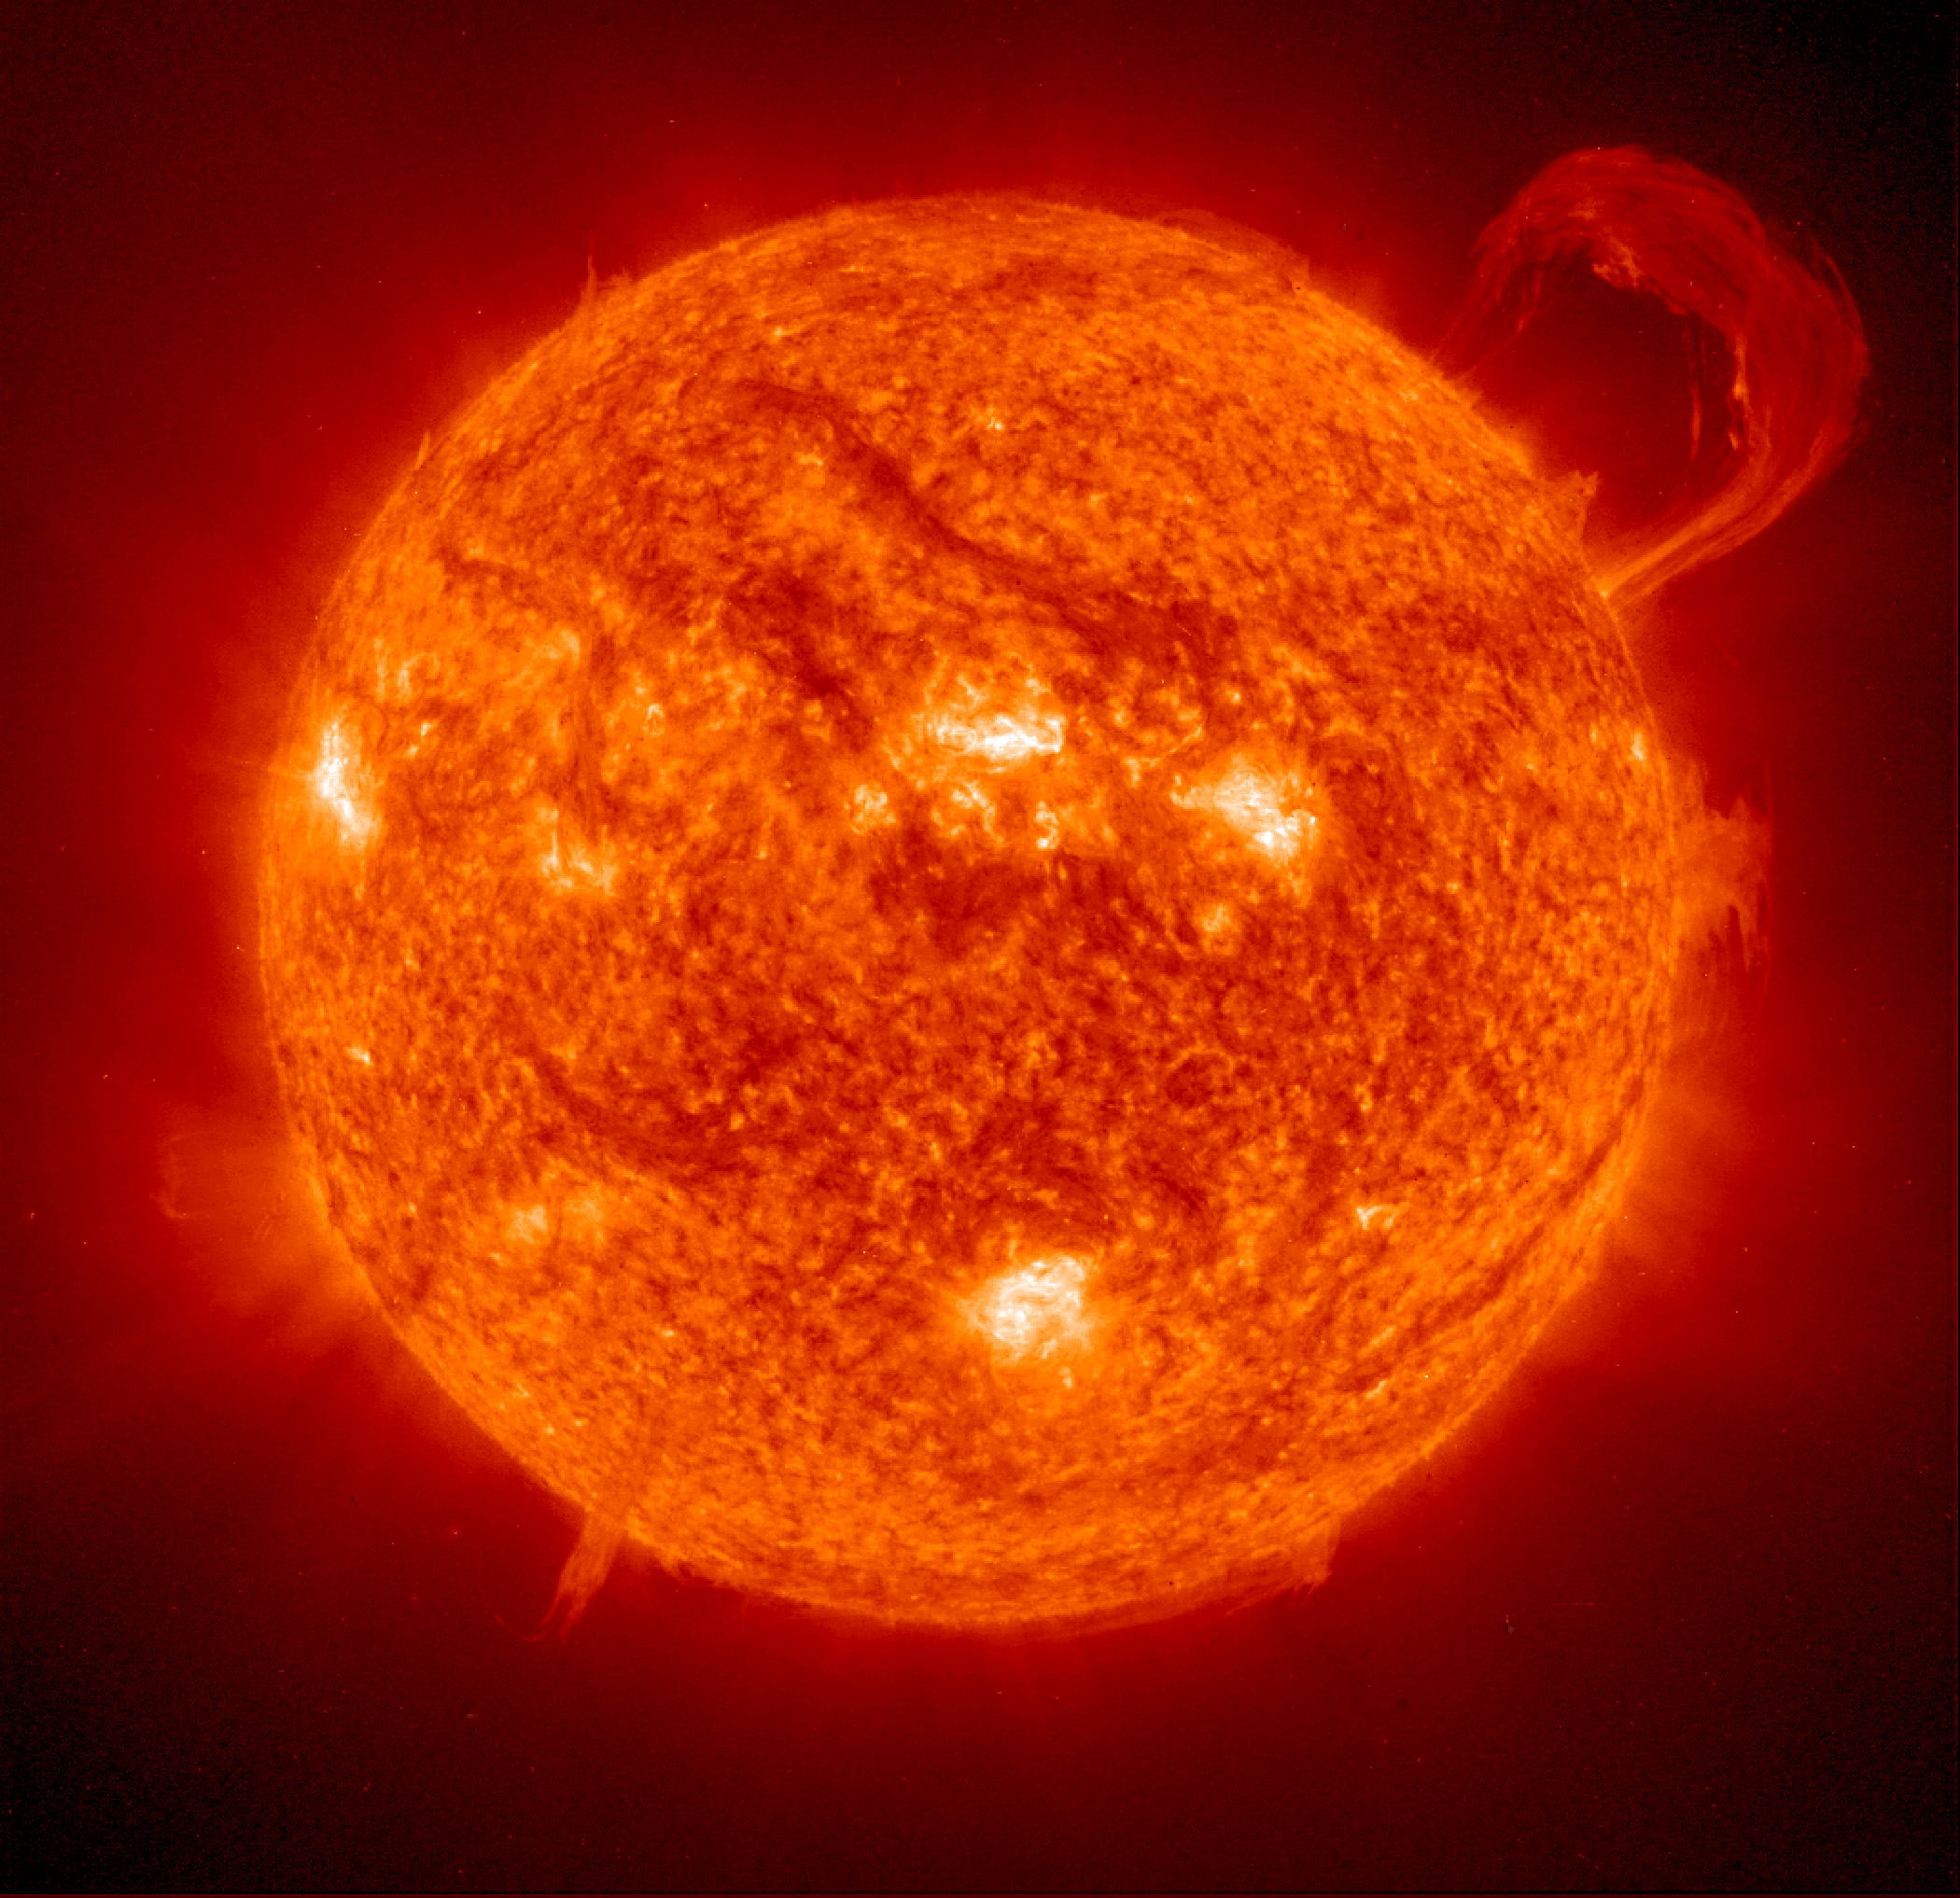
\includegraphics[width=0.5\textwidth]{Sun.jpg}
        \caption{Sol}
        \label{Sol}
    \end{figure}

El Modelo Estándar del sol, creado por astrofísicos durante los últimos 50 años, nos permite investigar muchas propiedades por separado. Una de ellas es la densidad del gas caliente en todo el interior. La función a continuación proporciona una fórmula de mejor ajuste, $D(x)$, para la densidad (en $\g/\cm^3$) desde el núcleo ($x=0$) hasta la superficie ($x=1$) y puntos intermedios.

$$D(x) = 519x^4 - 1630x^3 + 1844x^2 - 889x + 155$$

Por ejemplo, en un radio al $30\%$ del camino hacia la superficie, $x = 0.3$ y por lo tanto
$D(x=0.3) = 14.5 \g/\cm^3$.
\begin{enumerate}
	\item ¿Cuál es la densidad estimada del núcleo del sol?

	\item Al $1\%$ más cercano del radio del sol, ¿a qué radio la densidad del sol cae al $50\%$ de su densidad en el núcleo en $x=0$? 
	
	\item ¿Cuál es la densidad estimada del sol cerca de su superficie en $x=0.9$ usando esta aproximación polinómica?
\end{enumerate}
\end{problema}

\begin{problema}
El cohete Ares-V, que está siendo desarrollado actualmente por la NASA, pesará 3,700 toneladas en el despegue y podrá transportar 75 toneladas de suministros, equipos y hasta 4 astronautas a la luna. 

    \begin{figure}[H]
        \centering
        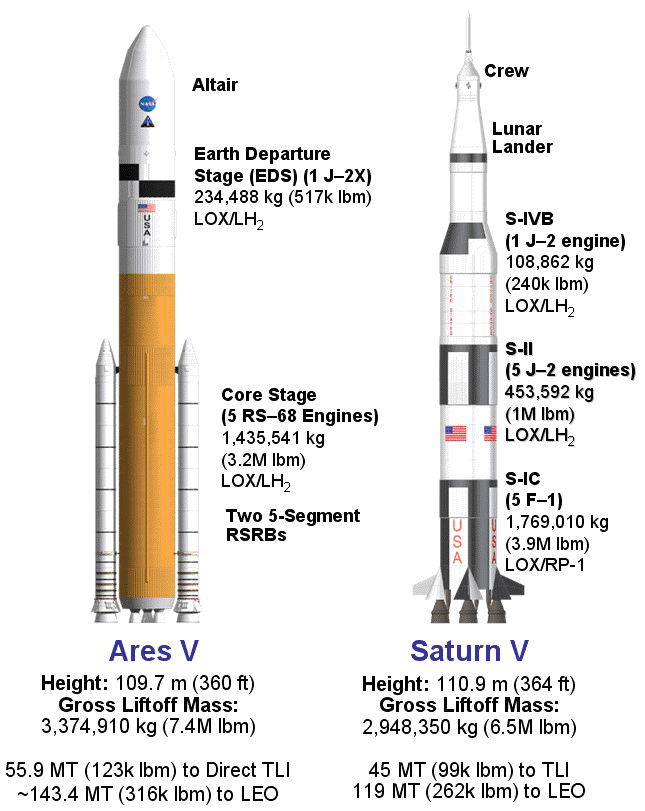
\includegraphics[width=0.5\textwidth]{AresVSaturnV.png}
        \caption{Ares V y Saturno V}
        \label{AresVSaturnV}
    \end{figure}

Como vehículo de lanzamiento de múltiples propósitos, también podrá lanzar cargas útiles científicas complejas y muy pesadas a Marte y más allá. Para hacer esto, los cohetes de la Etapa Central y los Cohetes de Combustible Sólido (SRBs) entregan un empuje combinado de 47 millones de Newtons. Para el cohete, definamos:

$T(t) = \text{empuje en el tiempo t}$
$m(t) = \text{masa en el tiempo t}$
$a(t) = \text{aceleración en el tiempo t}$

de modo que:

$a(t) = \frac{T(t)}{m(t)}$

El lanzamiento toma $200$ segundos. Supongamos que en el intervalo de tiempo $[0,200]$, $T(t)$ y $m(t)$ se dan aproximadamente de la siguiente manera:

$$T(x) = 8x^3 - 16x^2 - x^4 + 47$$

$$m(x) = 35 - x^2$$

donde $t = 40x$ 

Donde hemos usado un cambio de variable, de $t$ a $x$ para simplificar la forma de las ecuaciones.

\begin{enumerate}
	\item Grafica la curva de empuje $T(x)$ y la curva de masa $m(x)$ y encuentra todos los mínimos, máximos y puntos de inflexión en el intervalo $[0, 5]$.

	\item Grafica la curva de aceleración $a(x)$ y encuentra todos los máximos, mínimos y puntos de inflexión en el intervalo $[0, 5]$.

	\item ¿Para qué valor de $x$ la aceleración del cohete será máxima en el intervalo $[0, 5]$? ¿Cuántos segundos después del lanzamiento será esto?
\end{enumerate}

\end{problema}

\begin{problema}

Desde la década de 1930, los físicos saben que el "vacío" del espacio no está vacío. Contiene partículas y energía que aparecen y desaparecen, y no pueden ser detectadas directamente. Momentos después del Big Bang, esta energía del vacío fue lo suficientemente grande como para que, por sí misma, pudiera hacer que el universo se expandiera billones de veces en tamaño. Los astrónomos llaman a esto Inflación Cosmológica.

    \begin{figure}[H]
        \centering
        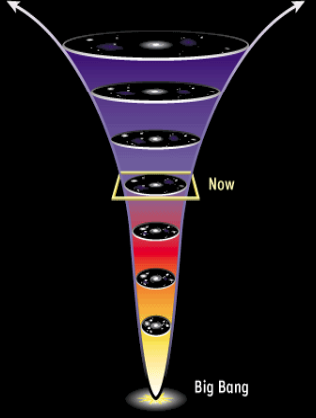
\includegraphics[width=0.5\textwidth]{BigBang.png}
        \caption{Big Bang}
        \label{BigBang}
    \end{figure}


Varios estudios teóricos del estado de vacío han centrado su atención en una función polinómica:

$$V(x) = \frac{L}{6} x^4 - m^2 x^2$$

Esta función, llamada Potencial de Coleman-Weinberg, permite a los físicos calcular la energía del estado de vacío, $V(x)$, en términos de la masa, $x$, de un nuevo tipo de partícula aún por descubrir llamada el X-Bosón.

\begin{enumerate}
	\item Factoriza $V(x)$ y determina la ubicación de todas las intersecciones con el eje x para el caso general donde $m$ y $L$ no están especificados.

	\item Para el caso específico de $V(x)$ donde $m=5$ y $L=6$, determina sus intersecciones con el eje x.

	\item Grafica $V(x)$ para $m=5$ y $L=6$ trazando una selección de puntos entre las intersecciones con el eje x.

	\item ¿Cuál es el comportamiento final (end behavior) de $V(x)$ para los valores seleccionados de $m$ y $L$?

	\item Usa una calculadora gráfica para encontrar el máximo relativo y los mínimos relativos para $V(x)$ con $m=5$ y $L=6$.
\end{enumerate}


\end{problema}



\cite{algebra2}
\bibliographystyle{plainurl}
\bibliography{bibliografia} % Nombre del .bib

\end{document}
